\pdfoptionpdfminorversion=5


% use this one if you want to have all the overlays
\documentclass{beamer}

% use this one if you want the slides without any overlays/transitions
% \documentclass[handout]{beamer}

% use this one if you want handouts with lines for notes next to them
% \documentclass[handout]{beamer}
% \usepackage{handoutWithNotes}
% \pgfpagesuselayout{2 on 1 with notes landscape}[letterpaper,border shrink=5mm]
% \pgfpagesuselayout{3 on 1 with notes}[letterpaper,border shrink=5mm]


\makeatletter
\@addtoreset{subfigure}{figure}
\makeatother

\usepackage[utf8x]{inputenc}
%\usepackage{default}

\usetheme{Antibes}
% \usetheme{Malmoe}

% \setbeamercovered{dynamic}

% trying to fix font warnings:
%\usepackage[utf8]{inputenc}
\usepackage[T1]{fontenc}
\usepackage{lmodern}
\usepackage{amsfonts}
\usepackage{amsmath}
\usepackage{amssymb}
\usepackage{type1cm} % fonts used by xfig generated figures needs that

\usepackage{multirow}

% \usepackage{subfigure}
% \usepackage{subfig}




% % Definition for subfloat to allow us to use listings/verbatim inside subfigures:
% \newbox\subfigbox % Create a box to hold the subfigure. 
% \makeatletter 
% \newenvironment{subfloat}% % Create the new environment. 
% {\def\caption##1{\gdef\subcapsave{\relax##1}}% 
% \let\subcapsave=\@empty % Save the subcaption text. 
% \let\sf@oldlabel=\label 
% \def\label##1{\xdef\sublabsave{\noexpand\label{##1}}}% 
% \let\sublabsave\relax % Save the label key. 
% \setbox\subfigbox\hbox 
% \bgroup}% % Open the box... 
% {\egroup % ... close the box and call \subfigure. 
% \let\label=\sf@oldlabel 
% \subfigure[\subcapsave]{\box\subfigbox}}% 
% \makeatother 



\usepackage{tikz}
\usepackage{tkz-graph}

\usetikzlibrary{arrows,%
                shapes,positioning}
\tikzstyle{node}=[circle,draw=blue!50!black!50,top color=white,bottom color=blue!50!black!25]
\tikzstyle{mynode}=[circle,draw=red!50!black!50,top color=white,bottom color=blue!50!black!25]
% \tikzstyle{user}=[ellipse,draw=green!50!black!50,top color=white,bottom color=green!50!black!25,densely dotted]
\tikzstyle{invis}=[draw=none]
% \tikzstyle{bisect}=[draw=red!50!black!50]


\author{Lloyd Brown}
\title{High-Performance Computing Networks at BYU}
\date{October 10, 2013}


\begin{document}

\frame{\titlepage}

\section*{Slide Download}
  \frame{
    \frametitle{Slide Download}

    To download these slides, use the following link:

    \begin{center}

      \url{http://goo.gl/IPRbEq}
      \begin{figure}
	\includegraphics{download_qr}
      \end{figure}

    \end{center}
    
}


\section{Outline}

  \frame{
    \tableofcontents
  }



\section{HPC Introduction}



\subsection{What is HPC?}

  \frame{
    \frametitle{What makes a supercomputer, super?}

    HPC or High-Performance Computing, is characterized by workloads and hardware requirements

    \begin{itemize}
      \pause\item Significantly larger compute capability than an average system
      \pause\item Used to solve problems that are too large to easily be solved on a single, traditional system
      \pause\item May utilize specialty hardware and software
      \pause\item No specific threshold for capacity
    \end{itemize}
  }

\subsection{Types of HPC}
  \frame{
    \frametitle{Nature of HPC Computing}
    In HPC, speedup comes from one of two sources:
    
    \begin{itemize}
      \pause\item Using faster resources (eg. faster clock speeds)
      \pause\item Using more resources (eg. using more processors) or \emph{Parallelism}
    \end{itemize}

    \pause Physics generally limits us on the faster resources, so we spend more time on parallelism.

  }

  \frame{
    \frametitle{Parallelism and Communication Needs}

    \begin{itemize}
      \item When utilizing multiple resources (eg. multiple processors), the program must:
      \begin{itemize}
	\pause\item Split up the workload
	\pause\item Provide necessary coordination among resources
      \end{itemize}
      \pause\item The algorithm and data determine the nature of communication needs
      \pause\item Therefore for HPC problems, communication is key.
      \begin{itemize}
	\pause\item For inter-process communication
	\pause\item For communicating with data storage
      \end{itemize}
    \end{itemize}

  }

%   \frame{
%     \frametitle{What kinds of HPC systems are out there?}
%     There are two major categories of HPC systems:
%     \begin{itemize}
%       \pause\item Systems which utilize specialty hardware, including:
%       \begin{itemize}
% 	\pause\item Processors
% 	\begin{itemize}
% 	  \pause\item Vector Processors (eg. Cray)
% 	  \pause\item Specialty Serial Processors (eg. Itanium, Power5, etc.)
% 	\end{itemize}
% 	\pause\item Accelerators
% 	\begin{itemize}
% 	  \pause\item Manycore (GPU \& Intel MIC)
% 	  \pause\item FPGA
% 	  \pause\item Cell
% 	\end{itemize}
% 	\pause\item Specialty/Proprietary Interconnects
% 	\begin{itemize}
% 	  \pause\item Infiniband
% 	  \pause\item NUMALink
% 	\end{itemize}
% % (eg. NUMALink, Infiniband, Quadrics, Myrinet, etc.)
%       \end{itemize}
%       \pause\item Commodity Hardware:
%       \begin{itemize}
% 	\pause\item Stock processors (eg. x86, x86\_64)
% 	\pause\item Stock interconnects (Ethernet)
%       \end{itemize}
%     \end{itemize}
% 
%   }
% 
% 
% 
% 
% 
\section{Types of Communication}
  \frame{
    \frametitle{What kind of communication are we talking about?}
    \begin{itemize}
      \pause\item Programs that utilize multiple processors to split up work, need to communicate between threads or processes, to coordinate efforts, report on results, etc.
      \pause\item Communication between threads/processes on the same host (``\emph{Intra}-node'' communication) is extremely fast (usually via shared memory)
      \pause\item If the processes are on different hosts, we have to go out to some communication fabric (``\emph{Inter}-node'' communication)
      \begin{itemize}
	\pause\item There's a lot of research in speeding up \emph{intra}-node communication, but that's more of a Computer Science or Electrical Engineering problem.  We'll spend our time today on \emph{inter}-node communication
      \end{itemize}
    \end{itemize}

  }
  
%   \frame{
%     \frametitle{Technologies for \emph{inter}-node communication}
%     Examples of technologies for \emph{inter}-node communication include:
%     \begin{itemize}
%       \pause\item Ethernet
%       \pause\item Fibre Channel
%       \pause\item WiFi (IEEE 802.11)
%       \pause\item Token Ring
%       \pause\item RS-232
%       \pause\item Infiniband
%     \end{itemize}
% 
%   }


\section{Infiniband}

  \frame{
    \frametitle{What is Infiniband?  And why do I care?}
    Infiniband is the most common high-performance interconnect used in HPC.  It:
    \begin{itemize}
      \pause\item is switched-fabric architecture (more like Fibre Channel than like Ethernet)
      \pause\item utilizes multiple speeds, lanes, and links
      \pause\item provides:
      \begin{itemize}
	\item extremely high bandwidth
	\pause\item extremely low latency (one-way < 5 $\mu$s, compared to approx. 22 $\mu$s for 1GbE)
      \end{itemize}
      \pause\item Speedup comes mostly from:
      \begin{itemize}
	\item Short protocol stack (very little above layer 2)
	\pause\item Low-latency switching (very little decision making in the switch)
	\pause\item Remote Direct Memory Access (RDMA)
      \end{itemize}
    \end{itemize}

  }

%   \subsection{Terminology}
% 
%   \frame{
%     \frametitle{Terms}
%     \begin{itemize}
%       \pause\item[HCA] Host Channel Adapter - The interface device that connects a host to the network
%       \pause\item[GUID] Globally-unique Identifier; hardware address on each HCA or switch; like a MAC address
%       \pause\item[LID] Logical Identifier (address) assigned by the subnet manager to the HCA; kinda like an IP, but resides in the upper part of layer 2
%       \pause\item[SM] Subnet Manager, a hardware or software device that assigns LIDs to GUIDs, and pre-loads the switch forwarding tables
%     \end{itemize}
% 
%   }

  \subsection{Physical Layer Characteristics}

  \frame{
    \frametitle{Lanes/Links/Speeds}
    Infiniband utilizes multiple lanes per physical link.  Each link has a certain speed based on the standard:

    \pause

    \begin{center}
     
      \begin{tabular}{|c|c|c|c|c|}
      \hline
		 & \emph{SDR} & \emph{DDR} & \emph{QDR} & \emph{FDR}\\
      \hline
      \emph{1x}  & 2.5 Gb/s & 5 Gb/s & 10 Gb/s & 14 Gb/s\\
      \hline
      \emph{4x}  & 10 Gb/s & 20 Gb/s & 40 Gb/s & 56 Gb/s\\
      \hline
      \emph{12x} & 30 Gb/s & 60 Gb/s & 120 Gb/s & 168 Gb/s\\
      \hline
      \end{tabular}
    \end{center}

  }
% % 
% % %   \frame{
% % %     \frametitle{Connectors}
% % %     
% % %   }
% % 
% %   \frame{
% %     \frametitle{Does this look familiar?}
% %     \begin{itemize}
% %       \item Is there any other common computer technology that looks like this from a physical layer?  Using multiple lanes, with per-lane speed doubling each successive iteration of the standard?\\
% % %     \pause Any gamers in the room?
% % %     \pause What is the most bandwidth and latency sensitive hardware used for gaming?  Requires the fastest communication?
% % %     \pause How about PCIe?
% %     
% % 	
% % 
% % %       \pause\centering{How about}\centering{\pause\strong{PCIe}}
% %       \pause\item How about \emph{PCI-Express}?
% %     \end{itemize}
% %   }
% % 
% % 
  \subsection{Encoding}
    \frame{
      \frametitle{Encoding Overhead}

      Infiniband uses bit-line encodings to guarantee bit transitions for clock synchronization:
      \begin{itemize}
	\item SDR, DDR, QDR - 8b/10b encoding (8 data bytes encoded in 10 bytes total; 20\% overhead)
	\item FDR and beyond - 64b/66b encoding (64 data bytes encoded in 66 bytes total; 3\% overhead)
      \end{itemize}



      \pause
      \begin{small}
      \begin{center}
      
	\begin{tabular}{|c|c|c|c|c|}
	\hline
		                    & \emph{SDR}   & \emph{DDR}  & \emph{QDR}	& \emph{FDR}\\
	\hline
	\multirow{2}{*}{\emph{1x}}  & 2.5 Gb/s raw & 5 Gb/s raw  & 10 Gb/s raw	& 14 Gb/s raw\\
				    & 2 Gb/s net   & 4 Gb/s net  & 8 Gb/s net  	& 13.6 Gb/s net\\
	\hline
	\multirow{2}{*}{\emph{4x}}  & 10 Gb/s raw  & 20 Gb/s raw & 40 Gb/s raw	& 56 Gb/s raw\\
				    & 8 Gb/s net   & 16 Gb/s net & 32 Gb/s net 	& 54.3 Gb/s net\\
	\hline
	\multirow{2}{*}{\emph{12x}} & 30 Gb/s raw  & 60 Gb/s raw & 120 Gb/s raw	& 168 Gb/s raw\\
				    & 24 Gb/s net  & 48 Gb/s net & 96 Gb/s net	& 162.9 Gb/s net\\
	\hline
	\end{tabular}
      \end{center}
      \end{small}
    }


  \subsection{Measured Performance}

  \frame{
    \frametitle{Performance at BYU's FSL}
    The graphs shown in the next couple of slides represent the bandwidth and latency performance of 4xQDR Infiniband vs 1Gb/s Ethernet at the Fulton Supercomputing Lab.

    \begin{itemize}
      \item All tests were performed host-to-host with one intervening switch (eg. host-switch-host)
      \item All tests utilize increasing message sizes, to demonstrate where one effect ends and the other starts
      \item Tests were performed using the ``osu\_bw'' and ``osu\_latency'' binaries from the OSU Micro-Benchmarks for MPI (a.k.a. ``OMB'')\footnote{\url{http://mvapich.cse.ohio-state.edu/benchmarks/}}
    \end{itemize}

  }

  \subsubsection{Bandwidth Comparison}

    \frame{
      \begin{figure}
	\includegraphics[scale=0.85]{IB_vs_Eth_Bandwidth.pdf}
      \end{figure}

    }

  \subsubsection{Latency Comparison}
    \frame{
      \begin{figure}
	\includegraphics[scale=0.85]{IB_vs_Eth_latency.pdf}
      \end{figure}

    }


  \subsection{Subnet Management}

    \frame{
      \frametitle{How Infiniband is Managed}
      Infiniband is designed as a trusted network.  The network is managed by a \emph{subnet manager} which does the following:
      \begin{itemize}
	\pause\item Periodically sweep the network, looking for topology changes, checking for errors, etc.
	\pause\item Build a cohesive model of the network topology
	\pause\item Load the switch forwarding tables with the LID/Port mapping
      \end{itemize}

    }

\section{Topologies}
    \frame{
      \frametitle{Infiniband Topologies}
      Infiniband puts very little restriction on the physical topology of the network.  
      \begin{itemize}
	\item<1-> The Subnet Manager loads all the forwarding tables into the switches
	\begin{itemize}
	  \item<2-> as long as you can build an appropriate graph parsing algorithm, and implement it in a subnet manager, you can use a topology
	  \item<3-> allows some much more interesting topologies than those commonly Ethernet and TCP/IP networks usually use.\footnote<3->{Technically you can use any topology with Ethernet as well.  It just takes a huge amount of very-messy work, for very little benefit.  I don't recommend trying it.}
	\end{itemize}
      \end{itemize}


    }


    \frame{
      \frametitle{Possible Topologies}
      \begin{itemize}
	\pause\item Tree/Fat-Tree
	\pause\item Fully-connected Mesh
% 	\pause\item Rectangular Mesh
	\pause\item Torus
	\pause\item Hypercube
	\pause\item Folded-Clos Network
      \end{itemize}


    }



    \frame{
      \frametitle{Fat Tree Example}
      A \emph{Fat Tree} is basically a tree with increased bandwidth (faster links or more links) between upper tiers relative to lower tiers; Ethernet has no problems with this one, so it's not terribly exciting
      \begin{center}
	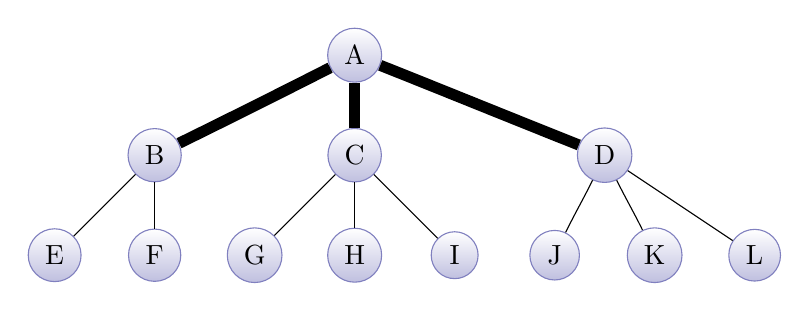
\begin{tikzpicture}[>=latex,line join=bevel,scale=0.5]
	%%
	\node (A) at (243bp,162bp) [node] {A};
	  \node (C) at (243bp,90bp) [node] {C};
	  \node (B) at (99bp,90bp) [node] {B};
	  \node (E) at (27bp,18bp) [node] {E};
	  \node (D) at (423bp,90bp) [node] {D};
	  \node (G) at (171bp,18bp) [node] {G};
	  \node (F) at (99bp,18bp) [node] {F};
	  \node (I) at (315bp,18bp) [node] {I};
	  \node (H) at (243bp,18bp) [node] {H};
	  \node (K) at (459bp,18bp) [node] {K};
	  \node (J) at (387bp,18bp) [node] {J};
	  \node (L) at (531bp,18bp) [node] {L};
	  \draw [] (C) ..controls (216bp,63bp) and (199bp,46bp)  .. (G);
	  \draw [] (D) ..controls (437bp,61bp) and (445bp,47bp)  .. (K);
	  \draw [] (C) ..controls (243bp,61bp) and (243bp,47bp)  .. (H);
	  \draw [] (D) ..controls (409bp,61bp) and (401bp,47bp)  .. (J);
	  \draw [] (C) ..controls (270bp,63bp) and (287bp,46bp)  .. (I);
	  \draw [] (D) ..controls (462bp,64bp) and (492bp,44bp)  .. (L);
	  \draw [line width=4bp] (A) ..controls (301bp,139bp) and (365bp,113bp)  .. (D);
	  \draw [] (B) ..controls (99bp,61bp) and (99bp,47bp)  .. (F);
	  \draw [line width=4bp] (A) ..controls (194bp,137bp) and (148bp,114bp)  .. (B);
	  \draw [] (B) ..controls (72bp,63bp) and (55bp,46bp)  .. (E);
	  \draw [line width=4bp] (A) ..controls (243bp,133bp) and (243bp,119bp)  .. (C);
	%

	%
	\end{tikzpicture}

      \end{center}
    }

  \frame{
    \frametitle{Fully-connected Mesh Example}
    \begin{itemize}
      \item<1->Pro: Shortest hop-count (1 hop) from any point to any other point
      \item<2->Con: takes a huge amount of cables, and the cable count increases very, very quickly.
    \end{itemize}

    \begin{center}
	
	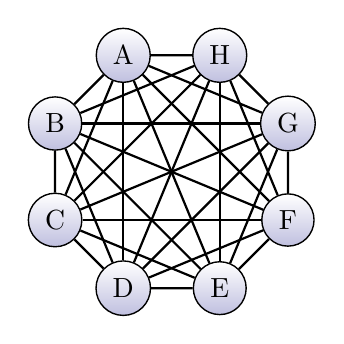
\begin{tikzpicture}[>=latex,line join=bevel,scale=1.6]
% 	  \node (A) at (336bp,81bp) [node] {A};
% 	  \node (C) at (108bp,41bp) [node] {C};
% 	  \node (B) at (378bp,197bp) [node] {I};
% 	  \node (E) at (28bp,259bp) [node] {E};
% 	  \node (D) at (28bp,135bp) [node] {D};
% 	  \node (G) at (229bp,375bp) [node] {G};
% 	  \node (F) at (108bp,353bp) [node] {F};
% 	  \node (I) at (229bp,19bp) [node] {B};
% 	  \node (H) at (336bp,313bp) [node] {H};
% 	  \draw [] (D) -- (H);
% 	  \draw [] (E) -- (F);
% % 	  \draw [] (E) -- (I);
% 	  \draw [] (D) -- (G);
% % 	  \draw [] (C) -- (I);
% % 	  \draw [] (H) -- (I);
% 	  \draw [] (D) -- (E);
% 	  \draw [] (A) -- (F);
% % 	  \draw [] (G) -- (I);
% 	  \draw [] (B) -- (F);
% 	  \draw [] (C) -- (D);
% 	  \draw [] (A) -- (B);
% % 	  \draw [] (D) -- (I);
% 	  \draw [] (E) -- (H);
% 	  \draw [] (C) -- (H);
% 	  \draw [] (F) -- (G);
% 	  \draw [] (B) -- (G);
% 	  \draw [] (A) -- (E);
% 	  \draw [] (F) -- (H);
% 	  \draw [] (B) -- (C);
% 	  \draw [] (C) -- (G);
% 	  \draw [] (B) -- (H);
% 	  \draw [] (A) -- (D);
% % 	  \draw [] (A) -- (I);
% 	  \draw [] (B) -- (D);
% 	  \draw [] (C) -- (F);
% 	  \draw [] (E) -- (G);
% % 	  \draw [] (F) -- (I);
% 	  \draw [] (D) -- (F);
% 	  \draw [] (A) -- (C);
% % 	  \draw [] (B) -- (I);
% 	  \draw [] (A) -- (G);
% 	  \draw [] (A) -- (H);
% 	  \draw [] (G) -- (H);
% 	  \draw [] (B) -- (E);
% 	  \draw [] (C) -- (E);
%     %

      \GraphInit
      \Vertex[style=node,x=-0.383,y=0.924]{A}
      \Vertex[style=node,x=-0.924,y=0.383]{B}
      \Vertex[style=node,x=-0.924,y=-0.383]{C}
      \Vertex[style=node,x=-0.383,y=-0.924]{D}
      \Vertex[style=node,x=0.383,y=-0.924]{E}
      \Vertex[style=node,x=0.924,y=-0.383]{F}
      \Vertex[style=node,x=0.924,y=0.383]{G}
      \Vertex[style=node,x=0.383,y=0.924]{H}




      \Edge(A)(B)
      \Edge(A)(C)
      \Edge(A)(D)
      \Edge(A)(E)
      \Edge(A)(F)
      \Edge(A)(G)
      \Edge(A)(H)

      \Edge(B)(C)
      \Edge(B)(D)
      \Edge(B)(E)
      \Edge(B)(F)
      \Edge(B)(G)
      \Edge(B)(H)

      \Edge(C)(D)
      \Edge(C)(E)
      \Edge(C)(F)
      \Edge(C)(G)
      \Edge(C)(H)

      \Edge(D)(E)
      \Edge(D)(F)
      \Edge(D)(G)
      \Edge(D)(H)

      \Edge(E)(F)
      \Edge(E)(G)
      \Edge(E)(H)

      \Edge(F)(G)
      \Edge(F)(H)

      \Edge(G)(H)
    \end{tikzpicture}
  \end{center}
  }

  \frame{
%     \frametitle{Rectangular Mesh / Torus Example}
    \frametitle{Torus example}
    \begin{itemize}
      \item<1->Pro: Excellent for large topologies (no core switches to buy)
      \item<2->Con: Higher hop count than other options, depending on size and shape
      \item<3->Con: Less desirable bandwidth ratios (MBB to Client BW; discussed later)
    \end{itemize}

    \begin{center}
      \begin{figure}
% 	\subfigure[Rectangular]{
% 	  \begin{tikzpicture}[>=latex,line join=bevel,scale=0.9]
% 	    \GraphInit
%       %       \SetVertexNormal[VertexStyle]
% 	    \Vertex[x=0,y=3,style=node]{A}
% 	    \Vertex[x=1,y=3,style=node]{B}
% 	    \Vertex[x=2,y=3,style=node]{C}
% 	    \Vertex[x=3,y=3,style=node]{D}
% 	    \Vertex[x=0,y=2,style=node]{E}
% 	    \Vertex[x=1,y=2,style=node]{F}
% 	    \Vertex[x=2,y=2,style=node]{G}
% 	    \Vertex[x=3,y=2,style=node]{H}
% 	    \Vertex[x=0,y=1,style=node]{I}
% 	    \Vertex[x=1,y=1,style=node]{J}
% 	    \Vertex[x=2,y=1,style=node]{K}
% 	    \Vertex[x=3,y=1,style=node]{L}
% 	    \Vertex[x=0,y=0,style=node]{M}
% 	    \Vertex[x=1,y=0,style=node]{N}
% 	    \Vertex[x=2,y=0,style=node]{O}
% 	    \Vertex[x=3,y=0,style=node]{P}
% 	    \Edge(A)(B)
% 	    \Edge(A)(E)
% 	    \Edge(B)(F)
% 	    \Edge(B)(C)
% 	    \Edge(C)(G)
% 	    \Edge(C)(D)
% 	    \Edge(D)(H)
% 	    \Edge(E)(F)
% 	    \Edge(E)(I)
% 	    \Edge(F)(G)
% 	    \Edge(F)(J)
% 	    \Edge(G)(H)
% 	    \Edge(G)(K)
% 	    \Edge(H)(L)
% 	    \Edge(I)(J)
% 	    \Edge(I)(M)
% 	    \Edge(J)(K)
% 	    \Edge(J)(N)
% 	    \Edge(K)(L)
% 	    \Edge(K)(O)
% 	    \Edge(L)(P)
% 	    \Edge(M)(N)
% 	    \Edge(N)(O)
% 	    \Edge(O)(P)
% 	  \end{tikzpicture}
% 	}%end of subfigure
% 	\subfigure[Torus]{
	  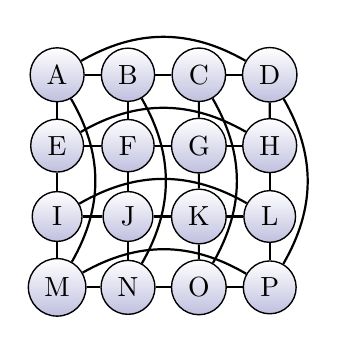
\begin{tikzpicture}[>=latex,line join=bevel,scale=0.9]
	    \GraphInit
      %       \SetVertexNormal[VertexStyle]
	    \Vertex[x=0,y=3,style=node]{A}
	    \Vertex[x=1,y=3,style=node]{B}
	    \Vertex[x=2,y=3,style=node]{C}
	    \Vertex[x=3,y=3,style=node]{D}
	    \Vertex[x=0,y=2,style=node]{E}
	    \Vertex[x=1,y=2,style=node]{F}
	    \Vertex[x=2,y=2,style=node]{G}
	    \Vertex[x=3,y=2,style=node]{H}
	    \Vertex[x=0,y=1,style=node]{I}
	    \Vertex[x=1,y=1,style=node]{J}
	    \Vertex[x=2,y=1,style=node]{K}
	    \Vertex[x=3,y=1,style=node]{L}
	    \Vertex[x=0,y=0,style=node]{M}
	    \Vertex[x=1,y=0,style=node]{N}
	    \Vertex[x=2,y=0,style=node]{O}
	    \Vertex[x=3,y=0,style=node]{P}
	    \Edge(A)(B)
	    \Edge(A)(E)
	    \Edge(B)(F)
	    \Edge(B)(C)
	    \Edge(C)(G)
	    \Edge(C)(D)
	    \Edge(D)(H)
	    \Edge(E)(F)
	    \Edge(E)(I)
	    \Edge(F)(G)
	    \Edge(F)(J)
	    \Edge(G)(H)
	    \Edge(G)(K)
	    \Edge(H)(L)
	    \Edge(I)(J)
	    \Edge(I)(M)
	    \Edge(J)(K)
	    \Edge(J)(N)
	    \Edge(K)(L)
	    \Edge(K)(O)
	    \Edge(L)(P)
	    \Edge(M)(N)
	    \Edge(N)(O)
	    \Edge(O)(P)

	    \Edge[style=bend right](D)(A)
	    \Edge[style=bend right](H)(E)
	    \Edge[style=bend right](L)(I)
	    \Edge[style=bend right](P)(M)
	    \Edge[style=bend right](M)(A)
	    \Edge[style=bend right](N)(B)
	    \Edge[style=bend right](O)(C)
	    \Edge[style=bend right](P)(D)
	  \end{tikzpicture}
% 	}%end of subfigure
      \end{figure}
    \end{center}
  }

  \frame{
    \frametitle{Hypercube example (4-dimensional)\footnote{Note that this is really just a special case of a Torus.}}
    \begin{itemize}
      \item<1->Pro: for \emph{d} dimensions, no more than \emph{d} hops from any other point in the topology
      \item<2->Con: cables/ports at each endpoint increase linearly with the dimension
    \end{itemize}


    \begin{center}
      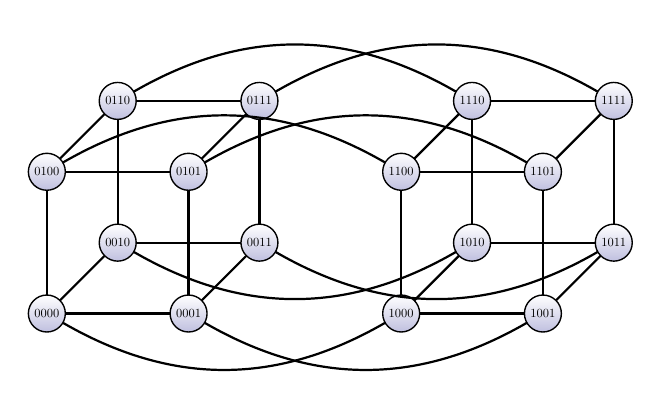
\begin{tikzpicture}[>=latex,line join=bevel,transform shape,scale=0.45]
	\GraphInit
	\Vertex[x=0,y=0,style=node]{0000}
	\Vertex[x=4,y=0,style=node]{0001}
	\Vertex[x=2,y=2,style=node]{0010}
	\Vertex[x=6,y=2,style=node]{0011}
	\Vertex[x=0,y=4,style=node]{0100}
	\Vertex[x=4,y=4,style=node]{0101}
	\Vertex[x=2,y=6,style=node]{0110}
	\Vertex[x=6,y=6,style=node]{0111}
	\Vertex[x=10,y=0,style=node]{1000}
	\Vertex[x=14,y=0,style=node]{1001}
	\Vertex[x=12,y=2,style=node]{1010}
	\Vertex[x=16,y=2,style=node]{1011}
	\Vertex[x=10,y=4,style=node]{1100}
	\Vertex[x=14,y=4,style=node]{1101}
	\Vertex[x=12,y=6,style=node]{1110}
	\Vertex[x=16,y=6,style=node]{1111}

	\Edge(0000)(0001)
	\Edge(0000)(0010)
	\Edge(0000)(0100)
	\Edge(0001)(0011)
	\Edge(0001)(0101)
	\Edge(0010)(0110)
	\Edge(0010)(0011)
	\Edge(0011)(0111)
	\Edge(0101)(0111)
	\Edge(0110)(0111)
	\Edge(0100)(0101)
	\Edge(0100)(0110)
	

	\Edge(1000)(1001)
	\Edge(1000)(1010)
	\Edge(1000)(1100)
	\Edge(1001)(1011)
	\Edge(1001)(1101)
	\Edge(1010)(1110)
	\Edge(1010)(1011)
	\Edge(1011)(1111)
	\Edge(1101)(1111)
	\Edge(1110)(1111)
	\Edge(1100)(1101)
	\Edge(1100)(1110)


	\Edge[style=bend right](0000)(1000)
	\Edge[style=bend right](0001)(1001)
	\Edge[style=bend right](0010)(1010)
	\Edge[style=bend right](0011)(1011)
	\Edge[style=bend left](0100)(1100)
	\Edge[style=bend left](0101)(1101)
	\Edge[style=bend left](0110)(1110)
	\Edge[style=bend left](0111)(1111)

      \end{tikzpicture}
    \end{center}

  }
  \frame{
    \frametitle{Folded Clos Network Example}
    \begin{center}
      \begin{itemize}
	\item Pros:
	\begin{itemize}
	  \item<1->Most common approach for small or medium-scale Infiniband fabrics
	  \item<2->Well understood (how larger IB switches are designed internally)
	  \item<3->Redundant; 1 link from each leaf to each spine
	  \item<4->Easy to expand (up to the port count of the switches)
	\end{itemize}
	\item<5->Con: Scalability limited by the port count of spine \& leaf switches
      \end{itemize}

      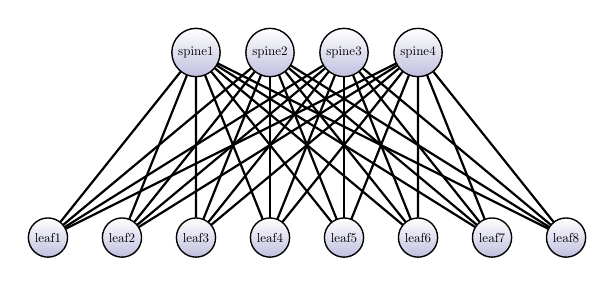
\begin{tikzpicture}[>=latex,line join=bevel,transform shape,scale=0.47]
	\GraphInit
	\Vertex[y=0,x=-3,style=node,L=spine1]{s1}
	\Vertex[y=0,x=-1,style=node,L=spine2]{s2}
	\Vertex[y=0,x=1,style=node,L=spine3]{s3}
	\Vertex[y=0,x=3,style=node,L=spine4]{s4}

	\Vertex[y=-5,x=-7,style=node,L=leaf1]{l1}
	\Vertex[y=-5,x=-5,style=node,L=leaf2]{l2}
	\Vertex[y=-5,x=-3,style=node,L=leaf3]{l3}
	\Vertex[y=-5,x=-1,style=node,L=leaf4]{l4}
	\Vertex[y=-5,x=1,style=node,L=leaf5]{l5}
	\Vertex[y=-5,x=3,style=node,L=leaf6]{l6}
	\Vertex[y=-5,x=5,style=node,L=leaf7]{l7}
	\Vertex[y=-5,x=7,style=node,L=leaf8]{l8}
	

	\Edge(s1)(l1)
	\Edge(s1)(l2)
	\Edge(s1)(l3)
	\Edge(s1)(l4)
	\Edge(s1)(l5)
	\Edge(s1)(l6)
	\Edge(s1)(l7)
	\Edge(s1)(l8)


	\Edge(s2)(l1)
	\Edge(s2)(l2)
	\Edge(s2)(l3)
	\Edge(s2)(l4)
	\Edge(s2)(l5)
	\Edge(s2)(l6)
	\Edge(s2)(l7)
	\Edge(s2)(l8)


	\Edge(s3)(l1)
	\Edge(s3)(l2)
	\Edge(s3)(l3)
	\Edge(s3)(l4)
	\Edge(s3)(l5)
	\Edge(s3)(l6)
	\Edge(s3)(l7)
	\Edge(s3)(l8)


	\Edge(s4)(l1)
	\Edge(s4)(l2)
	\Edge(s4)(l3)
	\Edge(s4)(l4)
	\Edge(s4)(l5)
	\Edge(s4)(l6)
	\Edge(s4)(l7)
	\Edge(s4)(l8)
      \end{tikzpicture}
    \end{center}

  }

  \frame{
    \frametitle{BYU Supercomputing's Clos Network}

    Note that this only shows the switches involved; there are 16 hosts attached to each leaf switch.

    \begin{center}
      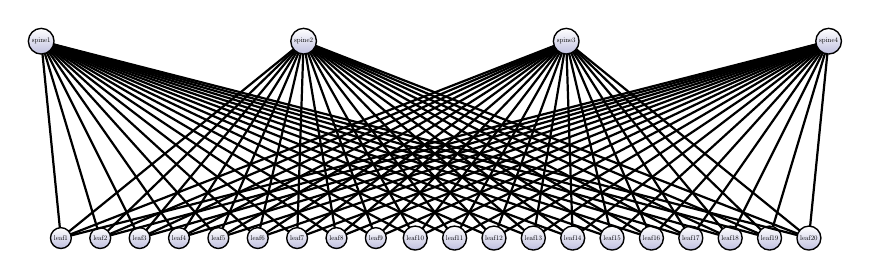
\begin{tikzpicture}[>=latex,line join=bevel,transform shape,scale=0.25]
	\GraphInit

	\Vertex[y=0,x=-20,style=node,L=spine1]{s1}
	\Vertex[y=0,x=-6.67,style=node,L=spine2]{s2}
	\Vertex[y=0,x=6.67,style=node,L=spine3]{s3}
	\Vertex[y=0,x=20,style=node,L=spine4]{s4}

% 	\Vertex[y=0,x=-17.5,style=node,L=spine1]{s1}
% 	\Vertex[y=0,x=-12.5,style=node,L=spine2]{s2}
% 	\Vertex[y=0,x=-7.5,style=node,L=spine3]{s3}
% 	\Vertex[y=0,x=-2.5,style=node,L=spine4]{s4}
% 	\Vertex[y=0,x=2.5,style=node,L=spine5]{s5}
% 	\Vertex[y=0,x=7.5,style=node,L=spine6]{s6}
% 	\Vertex[y=0,x=12.5,style=node,L=spine7]{s7}
% 	\Vertex[y=0,x=17.5,style=node,L=spine8]{s8}
% 
% 	\Vertex[y=-20,x=-20,style=node,L=leaf1]{l1}
% 	\Vertex[y=-20,x=-18,style=node,L=leaf2]{l2}
% 	\Vertex[y=-20,x=-16,style=node,L=leaf3]{l3}
% 	\Vertex[y=-20,x=-14,style=node,L=leaf4]{l4}
% 	\Vertex[y=-20,x=-12,style=node,L=leaf5]{l5}
% 	\Vertex[y=-20,x=-10,style=node,L=leaf6]{l6}
% 	\Vertex[y=-20,x=-8,style=node,L=leaf7]{l7}
% 	\Vertex[y=-20,x=-6,style=node,L=leaf8]{l8}
% 	\Vertex[y=-20,x=-4,style=node,L=leaf9]{l9}
% 	\Vertex[y=-20,x=-2,style=node,L=leaf10]{l10}
% 	\Vertex[y=-20,x=0,style=node,L=leaf11]{l11}
% 	\Vertex[y=-20,x=2,style=node,L=leaf12]{l12}
% 	\Vertex[y=-20,x=4,style=node,L=leaf13]{l13}
% 	\Vertex[y=-20,x=6,style=node,L=leaf14]{l14}
% 	\Vertex[y=-20,x=8,style=node,L=leaf15]{l15}
% 	\Vertex[y=-20,x=10,style=node,L=leaf16]{l16}
% 	\Vertex[y=-20,x=12,style=node,L=leaf17]{l17}
% 	\Vertex[y=-20,x=14,style=node,L=leaf18]{l18}
% 	\Vertex[y=-20,x=16,style=node,L=leaf19]{l19}
% 	\Vertex[y=-20,x=18,style=node,L=leaf20]{l20}
% 	\Vertex[y=-20,x=20,style=node,L=leaf21]{l21}
% 

	\Vertex[y=-10,x=-19,style=node,L=leaf1]{l1}
	\Vertex[y=-10,x=-17,style=node,L=leaf2]{l2}
	\Vertex[y=-10,x=-15,style=node,L=leaf3]{l3}
	\Vertex[y=-10,x=-13,style=node,L=leaf4]{l4}
	\Vertex[y=-10,x=-11,style=node,L=leaf5]{l5}
	\Vertex[y=-10,x=-9,style=node,L=leaf6]{l6}
	\Vertex[y=-10,x=-7,style=node,L=leaf7]{l7}
	\Vertex[y=-10,x=-5,style=node,L=leaf8]{l8}
	\Vertex[y=-10,x=-3,style=node,L=leaf9]{l9}
	\Vertex[y=-10,x=-1,style=node,L=leaf10]{l10}
	\Vertex[y=-10,x=1,style=node,L=leaf11]{l11}
	\Vertex[y=-10,x=3,style=node,L=leaf12]{l12}
	\Vertex[y=-10,x=5,style=node,L=leaf13]{l13}
	\Vertex[y=-10,x=7,style=node,L=leaf14]{l14}
	\Vertex[y=-10,x=9,style=node,L=leaf15]{l15}
	\Vertex[y=-10,x=11,style=node,L=leaf16]{l16}
	\Vertex[y=-10,x=13,style=node,L=leaf17]{l17}
	\Vertex[y=-10,x=15,style=node,L=leaf18]{l18}
	\Vertex[y=-10,x=17,style=node,L=leaf19]{l19}
	\Vertex[y=-10,x=19,style=node,L=leaf20]{l20}


	\Edge(s1)(l1)
	\Edge(s1)(l2)
	\Edge(s1)(l3)
	\Edge(s1)(l4)
	\Edge(s1)(l5)
	\Edge(s1)(l6)
	\Edge(s1)(l7)
	\Edge(s1)(l8)
	\Edge(s1)(l9)
	\Edge(s1)(l10)
	\Edge(s1)(l11)
	\Edge(s1)(l12)
	\Edge(s1)(l13)
	\Edge(s1)(l14)
	\Edge(s1)(l15)
	\Edge(s1)(l16)
	\Edge(s1)(l17)
	\Edge(s1)(l18)
	\Edge(s1)(l19)
	\Edge(s1)(l20)
% 	\Edge(s1)(l21)

	\Edge(s2)(l1)
	\Edge(s2)(l2)
	\Edge(s2)(l3)
	\Edge(s2)(l4)
	\Edge(s2)(l5)
	\Edge(s2)(l6)
	\Edge(s2)(l7)
	\Edge(s2)(l8)
	\Edge(s2)(l9)
	\Edge(s2)(l10)
	\Edge(s2)(l11)
	\Edge(s2)(l12)
	\Edge(s2)(l13)
	\Edge(s2)(l14)
	\Edge(s2)(l15)
	\Edge(s2)(l16)
	\Edge(s2)(l17)
	\Edge(s2)(l18)
	\Edge(s2)(l19)
	\Edge(s2)(l20)
% 	\Edge(s2)(l21)

	\Edge(s3)(l1)
	\Edge(s3)(l2)
	\Edge(s3)(l3)
	\Edge(s3)(l4)
	\Edge(s3)(l5)
	\Edge(s3)(l6)
	\Edge(s3)(l7)
	\Edge(s3)(l8)
	\Edge(s3)(l9)
	\Edge(s3)(l10)
	\Edge(s3)(l11)
	\Edge(s3)(l12)
	\Edge(s3)(l13)
	\Edge(s3)(l14)
	\Edge(s3)(l15)
	\Edge(s3)(l16)
	\Edge(s3)(l17)
	\Edge(s3)(l18)
	\Edge(s3)(l19)
	\Edge(s3)(l20)
% 	\Edge(s3)(l21)

	\Edge(s4)(l1)
	\Edge(s4)(l2)
	\Edge(s4)(l3)
	\Edge(s4)(l4)
	\Edge(s4)(l5)
	\Edge(s4)(l6)
	\Edge(s4)(l7)
	\Edge(s4)(l8)
	\Edge(s4)(l9)
	\Edge(s4)(l10)
	\Edge(s4)(l11)
	\Edge(s4)(l12)
	\Edge(s4)(l13)
	\Edge(s4)(l14)
	\Edge(s4)(l15)
	\Edge(s4)(l16)
	\Edge(s4)(l17)
	\Edge(s4)(l18)
	\Edge(s4)(l19)
	\Edge(s4)(l20)
% 	\Edge(s4)(l21)
% 
% 	\Edge(s5)(l1)
% 	\Edge(s5)(l2)
% 	\Edge(s5)(l3)
% 	\Edge(s5)(l4)
% 	\Edge(s5)(l5)
% 	\Edge(s5)(l6)
% 	\Edge(s5)(l7)
% 	\Edge(s5)(l8)
% 	\Edge(s5)(l9)
% 	\Edge(s5)(l10)
% 	\Edge(s5)(l11)
% 	\Edge(s5)(l12)
% 	\Edge(s5)(l13)
% 	\Edge(s5)(l14)
% 	\Edge(s5)(l15)
% 	\Edge(s5)(l16)
% 	\Edge(s5)(l17)
% 	\Edge(s5)(l18)
% 	\Edge(s5)(l19)
% 	\Edge(s5)(l20)
% 	\Edge(s5)(l21)
% 
% 	\Edge(s6)(l1)
% 	\Edge(s6)(l2)
% 	\Edge(s6)(l3)
% 	\Edge(s6)(l4)
% 	\Edge(s6)(l5)
% 	\Edge(s6)(l6)
% 	\Edge(s6)(l7)
% 	\Edge(s6)(l8)
% 	\Edge(s6)(l9)
% 	\Edge(s6)(l10)
% 	\Edge(s6)(l11)
% 	\Edge(s6)(l12)
% 	\Edge(s6)(l13)
% 	\Edge(s6)(l14)
% 	\Edge(s6)(l15)
% 	\Edge(s6)(l16)
% 	\Edge(s6)(l17)
% 	\Edge(s6)(l18)
% 	\Edge(s6)(l19)
% 	\Edge(s6)(l20)
% 	\Edge(s6)(l21)
% 
% 	\Edge(s7)(l1)
% 	\Edge(s7)(l2)
% 	\Edge(s7)(l3)
% 	\Edge(s7)(l4)
% 	\Edge(s7)(l5)
% 	\Edge(s7)(l6)
% 	\Edge(s7)(l7)
% 	\Edge(s7)(l8)
% 	\Edge(s7)(l9)
% 	\Edge(s7)(l10)
% 	\Edge(s7)(l11)
% 	\Edge(s7)(l12)
% 	\Edge(s7)(l13)
% 	\Edge(s7)(l14)
% 	\Edge(s7)(l15)
% 	\Edge(s7)(l16)
% 	\Edge(s7)(l17)
% 	\Edge(s7)(l18)
% 	\Edge(s7)(l19)
% 	\Edge(s7)(l20)
% 	\Edge(s7)(l21)
% 
% 	\Edge(s8)(l1)
% 	\Edge(s8)(l2)
% 	\Edge(s8)(l3)
% 	\Edge(s8)(l4)
% 	\Edge(s8)(l5)
% 	\Edge(s8)(l6)
% 	\Edge(s8)(l7)
% 	\Edge(s8)(l8)
% 	\Edge(s8)(l9)
% 	\Edge(s8)(l10)
% 	\Edge(s8)(l11)
% 	\Edge(s8)(l12)
% 	\Edge(s8)(l13)
% 	\Edge(s8)(l14)
% 	\Edge(s8)(l15)
% 	\Edge(s8)(l16)
% 	\Edge(s8)(l17)
% 	\Edge(s8)(l18)
% 	\Edge(s8)(l19)
% 	\Edge(s8)(l20)
% 	\Edge(s8)(l21)

      \end{tikzpicture}
    \end{center}

  }
% 
%   \subsection{Upper Layer Protocol Stack Components}
%     \frame{
%       \frametitle{Upper Layer Stack}
%       The protocol stack includes several optional components to enable application communication:
%       \begin{itemize}
% 	\pause\item[SRP] SCSI RDMA Protocol - Block Storage Protocol; competing with iSER
% 	\item[iSER] iSCSI extensions for RDMA - Block Storage Protocol; competing with SRP
% 	\pause\item[IPoIB] IP over Infiniband - not the most efficient, but works
% 	\pause\item[Verbs] Native IB API for general application use
% 	\pause\item[SDP] Sockets Direct Protocol - basically sockets protocol for IB
%       \end{itemize}
% 
%     }
% 
%     \frame{
%       \frametitle{Other (usu. Proprietary) Extensions}
% 	Other extensions exist, usually implemented in a proprietary fashion, including the following:
% 	\begin{itemize}
% 	  \pause\item[FCoIB] Fibre-Channel traffic over IB
% 	  \pause\item[ETHoIB] Ethernet over IB
% 	  \pause\item[FlexBoot] PXE-like network booting
% 	\end{itemize}
% 
%     }
% 
%     \frame{
%       \frametitle{Message Passing}
%       \begin{itemize}
% 	\item In HPC, most applications use a message-passing library like MPI, which in turn uses the Verbs API to do its work.
% 	\item Several dozen MPI implementations exist, but the most common that can utilize Infiniband are:
%       
% 	\begin{itemize}
% 	  \item OpenMPI
% 	  \item MVAPICH
% 	  \item Intel MPI
% 	  \item HP/Platform MPI
% 	\end{itemize}
%       \end{itemize}
% 
%     }
%   
%   \subsection{Other Considerations - Expense}
% 
%     \frame{
%       \frametitle{Costs}
%       In general:
%       \begin{itemize}
% 	\item Gigabit Ethernet comes on-board for most hosts, so it has very little cost
% 	\pause\item 10-Gigabit Ethernet is coming on-board for some hosts
% 	\pause\item Per-port cost for 4xQDR Infiniband (40 Gb/s) is usually less than 10-Gigabit Ethernet, but this changes over time
% 	\pause\item 4xQDR (40Gb/s) HCAs can be repurposed (via firmware change) to be 10-Gigabit Ethernet NICs
%       \end{itemize}
% 
%     }
% 
% 
% 
% 
% 
% % \section{Building your own HPC Cluster}
% % 
% %   \frame{
% %     \frametitle{Components needed to build an HPC Cluster}
% % 
% %     To build your own HPC cluster, consider the following components:
% % 
% %     \begin{itemize}
% % %       \pause\item System Hardware
% % %       \pause\item Network Hardware
% %       \pause\item Hardware
% %       \pause\item Operating System Software
% %       \pause\item Infrastructure Software
% %       \pause\item Computational Software
% %     \end{itemize}
% % 
% %   }
% % 
% %   \subsection{Hardware}
% %     \frame{
% %       \frametitle{Hardware Considerations}
% %       When considering system hardware, be aware of the following considerations:
% %       \begin{itemize}
% % 	\pause\item If a process is using resources on multiple nodes, it's significantly easier if the nodes' hardware is homogeneous.
% % 	\pause\item You need to know the task's or software's requirements, and build the system appropriately in the following areas:
% % 	\begin{itemize}
% % 	  \pause\item Processor features and speed
% % 	  \pause\item RAM
% % 	  \pause\item Network Performance (bandwidth and latency)
% % 	  \pause\item Storage requirements (total capacity, throughput, and IOPS)
% % 	\end{itemize}
% %       \end{itemize}
% % 
% %     }
% %   \subsection{OS Software}
% % 
% %     \frame{
% %       \frametitle{Compute Node Operating System}
% %       \begin{itemize}
% % 	\pause\item Each computational node needs to have a functioning operating system.  \emph{Linux} is the most common, usually installed either through a \emph{golden image} approach (usually vendor-provided), or scalable, scripted installer, eg. \emph{NPACI Rocks}.
% % 	\pause\item You will need to make sure your computational software is supported on the system.  For example, many more commercial software packages run on \emph{RedHat Enterprise Linux} than on \emph{Ubuntu}.
% %       \end{itemize}
% % 
% %     }
% % 
% %   \subsection{Infrastructure Software}
% %     \frame{
% %       \frametitle{Organizing the effort}
% %       \begin{itemize}
% % 	\pause\item If you're the only person using the system, you can just run your tasks directly.  If, however, you need to allow multiple users to have access, etc., you will probably need a queuing mechanism, eg. Moab/Torque, PBSPro, Slurm, SGE, LoadLeveler, LSF
% % 	\pause\item You will need to monitor the system for hardware and software failures.  Think something like \emph{ganglia}.
% %       \end{itemize}
% %     }
% % 
% %   \subsection{Computational Software}
% %     \frame{
% %       \frametitle{Actually doing work}
% %       In order for the system to be useful, you need software to do some calculations.  Some things to consider here:
% %       \begin{itemize}
% % 	\pause\item How will I get the software to utilize all the resources (eg. processors) available?  Do I need to use some form of communication framework like MPI to coordinate efforts, or will I just launch independent tasks
% % 	\pause\item Is there any form of tuning that I can do to make the software more efficient?  For example, if it's compiled software, am I taking advantage of compilation optimizations, eg. SSE, or specialty BLAS implementations like Intel MKL or GotoBlas?
% %       \end{itemize}
% % 
% %     }
% % 
% 
%   \section{Summary/Conclusions}
% 
%   \frame{
%     \frametitle{What does this all mean?}
%     \begin{itemize}
%       \pause\item In general, clusters of commodity hardware are the cheapest approaches to HPC, but it will vary depending on situation.
%       \pause\item It is possible to set up a small HPC cluster without much hardware cost, or any real software cost.  Just don't expect anything \"{u}ber-cool like Infiniband.
%       \pause\item You absolutely must understand your software, and its requirements
%       \pause\item Not everything works like Ethernet and TCP/IP.  Network technologies like Fibre Channel and Infiniband throw away a number of the basic assumptions of Ethernet.
%     \end{itemize}
%   }


  \subsection{Evaluating Topologies}
  \frame{
    \frametitle{What are some important characteristics for evaluating networks and topologies?}
    \begin{itemize}
	\pause\item Total host bandwidth
	\pause\item Latency/hop-count
	\pause\item Cost
	\pause\item Ease of expansion
	\pause\item Minimum Bisection Bandwidth
	\pause\item MBB to Client BW Ratio
    \end{itemize}
  }

  \frame{
    \frametitle{What's ``Minimum Bisection Bandwidth''?}
    \begin{itemize}
      \pause\item If you were to draw a line across a topology, such that half the clients/switches/whatever are on each side of the line, the total bandwidth of all the links ``cut'' by that line is the \emph{bisection bandwidth}
      \pause\item Of all the possible \emph{bisection bandwidth} lines, the one with the minimum bandwidth is called the \emph{minimum bisection bandwidth}
    \end{itemize}
  }


  \frame{
    \frametitle{MBB Example - Torus}
    
    Which bisection line represents the minimum bandwidth bisection (assume all links are the same speed)?
    \begin{itemize}
     \item<2-> \begin{small}Green line cuts 8 links; red line cuts 12 links; Green is the \emph{minimum}\end{small}
    \end{itemize}



    \begin{center}
      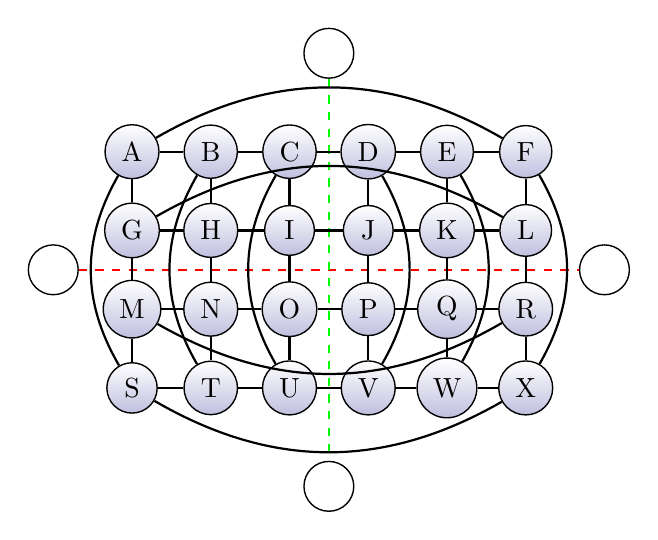
\begin{tikzpicture}[>=latex,line join=bevel,scale=1.0]
	    \GraphInit
      %       \SetVertexNormal[VertexStyle]
\Vertex[x=0,y=3,style=node]{A}
\Vertex[x=1,y=3,style=node]{B}
\Vertex[x=2,y=3,style=node]{C}
\Vertex[x=3,y=3,style=node]{D}
\Vertex[x=4,y=3,style=node]{E}
\Vertex[x=5,y=3,style=node]{F}
\Vertex[x=0,y=2,style=node]{G}
\Vertex[x=1,y=2,style=node]{H}
\Vertex[x=2,y=2,style=node]{I}
\Vertex[x=3,y=2,style=node]{J}
\Vertex[x=4,y=2,style=node]{K}
\Vertex[x=5,y=2,style=node]{L}
\Vertex[x=0,y=1,style=node]{M}
\Vertex[x=1,y=1,style=node]{N}
\Vertex[x=2,y=1,style=node]{O}
\Vertex[x=3,y=1,style=node]{P}
\Vertex[x=4,y=1,style=node]{Q}
\Vertex[x=5,y=1,style=node]{R}
\Vertex[x=0,y=0,style=node]{S}
\Vertex[x=1,y=0,style=node]{T}
\Vertex[x=2,y=0,style=node]{U}
\Vertex[x=3,y=0,style=node]{V}
\Vertex[x=4,y=0,style=node]{W}
\Vertex[x=5,y=0,style=node]{X}


% 	    \Edge(A)(B)
% 	    \Edge(A)(E)
% 	    \Edge(B)(F)
% 	    \Edge(B)(C)
% 	    \Edge(C)(G)
% 	    \Edge(C)(D)
% 	    \Edge(D)(H)
% 	    \Edge(E)(F)
% 	    \Edge(E)(I)
% 	    \Edge(F)(G)
% 	    \Edge(F)(J)
% 	    \Edge(G)(H)
% 	    \Edge(G)(K)
% 	    \Edge(H)(L)
% 	    \Edge(I)(J)
% 	    \Edge(I)(M)
% 	    \Edge(J)(K)
% 	    \Edge(J)(N)
% 	    \Edge(K)(L)
% 	    \Edge(K)(O)
% 	    \Edge(L)(P)
% 	    \Edge(M)(N)
% 	    \Edge(N)(O)
% 	    \Edge(O)(P)
% 
% 	    \Edge[style=bend right](D)(A)
% 	    \Edge[style=bend right](H)(E)
% 	    \Edge[style=bend right](L)(I)
% 	    \Edge[style=bend right](P)(M)
% 	    \Edge[style=bend right](M)(A)
% 	    \Edge[style=bend right](N)(B)
% 	    \Edge[style=bend right](O)(C)
% 	    \Edge[style=bend right](P)(D)

\Vertex[x=-1,y=1.5,style=invis,NoLabel=true]{Ihl}
\Vertex[x=6,y=1.5,style=invis,NoLabel=true]{Ihr}
\Vertex[x=2.5,y=-1.25,style=invis,NoLabel=true]{Ivb}
\Vertex[x=2.5,y=4.25,style=invis,NoLabel=true]{Ivt}
\SetUpEdge[color=red,style=dashed]
\Edge(Ihl)(Ihr)
\SetUpEdge[color=green,style=dashed]
\Edge(Ivt)(Ivb)

\SetUpEdge[color=black,style=]

\Edge(A)(B)
\Edge(B)(C)
\Edge(C)(D)
\Edge(D)(E)
\Edge(E)(F)
\Edge(G)(H)
\Edge(H)(I)
\Edge(I)(J)
\Edge(J)(K)
\Edge(K)(L)
\Edge(M)(N)
\Edge(N)(O)
\Edge(O)(P)
\Edge(P)(Q)
\Edge(Q)(R)
\Edge(S)(T)
\Edge(T)(U)
\Edge(U)(V)
\Edge(V)(W)
\Edge(W)(X)

\Edge(A)(G)
\Edge(G)(M)
\Edge(M)(S)
\Edge(B)(H)
\Edge(H)(N)
\Edge(N)(T)
\Edge(C)(I)
\Edge(I)(O)
\Edge(O)(U)
\Edge(D)(J)
\Edge(J)(P)
\Edge(P)(V)
\Edge(E)(K)
\Edge(K)(Q)
\Edge(Q)(W)
\Edge(F)(L)
\Edge(L)(R)
\Edge(R)(X)

\Edge[style=bend left](A)(F)
\Edge[style=bend left](G)(L)
\Edge[style=bend right](M)(R)
\Edge[style=bend right](S)(X)
\Edge[style=bend right](A)(S)
\Edge[style=bend right](B)(T)
\Edge[style=bend right](C)(U)
\Edge[style=bend left](D)(V)
\Edge[style=bend left](E)(W)
\Edge[style=bend left](F)(X)


	  \end{tikzpicture}
    \end{center}

  }

  \frame{
    \frametitle{Why is MBB important?}

    \begin{itemize}
      \pause\item MBB represents the available bandwidth during a worst-case scenario:
      \begin{itemize}
	\pause\item All the clients on one side of the MBB line are trying to communicate with someone on the other side of the line, as fast as possible
      \end{itemize}
    \end{itemize}
  }

  \frame{
    \frametitle{MBB Example - Torus}
    

    \begin{center}
      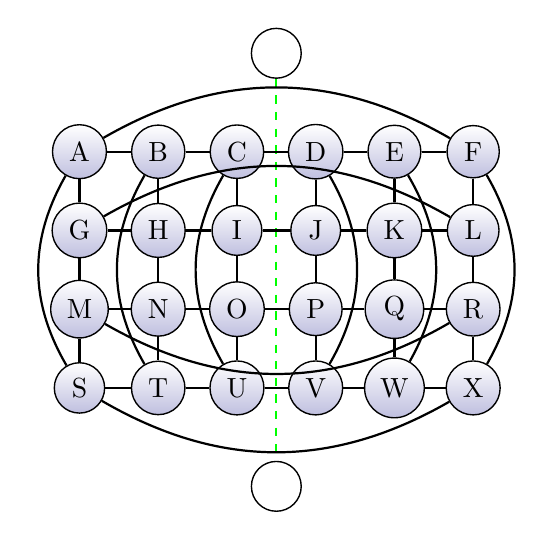
\begin{tikzpicture}[>=latex,line join=bevel,scale=1.0]
	    \GraphInit
      %       \SetVertexNormal[VertexStyle]
\Vertex[x=0,y=3,style=node]{A}
\Vertex[x=1,y=3,style=node]{B}
\Vertex[x=2,y=3,style=node]{C}
\Vertex[x=3,y=3,style=node]{D}
\Vertex[x=4,y=3,style=node]{E}
\Vertex[x=5,y=3,style=node]{F}
\Vertex[x=0,y=2,style=node]{G}
\Vertex[x=1,y=2,style=node]{H}
\Vertex[x=2,y=2,style=node]{I}
\Vertex[x=3,y=2,style=node]{J}
\Vertex[x=4,y=2,style=node]{K}
\Vertex[x=5,y=2,style=node]{L}
\Vertex[x=0,y=1,style=node]{M}
\Vertex[x=1,y=1,style=node]{N}
\Vertex[x=2,y=1,style=node]{O}
\Vertex[x=3,y=1,style=node]{P}
\Vertex[x=4,y=1,style=node]{Q}
\Vertex[x=5,y=1,style=node]{R}
\Vertex[x=0,y=0,style=node]{S}
\Vertex[x=1,y=0,style=node]{T}
\Vertex[x=2,y=0,style=node]{U}
\Vertex[x=3,y=0,style=node]{V}
\Vertex[x=4,y=0,style=node]{W}
\Vertex[x=5,y=0,style=node]{X}


% 	    \Edge(A)(B)
% 	    \Edge(A)(E)
% 	    \Edge(B)(F)
% 	    \Edge(B)(C)
% 	    \Edge(C)(G)
% 	    \Edge(C)(D)
% 	    \Edge(D)(H)
% 	    \Edge(E)(F)
% 	    \Edge(E)(I)
% 	    \Edge(F)(G)
% 	    \Edge(F)(J)
% 	    \Edge(G)(H)
% 	    \Edge(G)(K)
% 	    \Edge(H)(L)
% 	    \Edge(I)(J)
% 	    \Edge(I)(M)
% 	    \Edge(J)(K)
% 	    \Edge(J)(N)
% 	    \Edge(K)(L)
% 	    \Edge(K)(O)
% 	    \Edge(L)(P)
% 	    \Edge(M)(N)
% 	    \Edge(N)(O)
% 	    \Edge(O)(P)
% 
% 	    \Edge[style=bend right](D)(A)
% 	    \Edge[style=bend right](H)(E)
% 	    \Edge[style=bend right](L)(I)
% 	    \Edge[style=bend right](P)(M)
% 	    \Edge[style=bend right](M)(A)
% 	    \Edge[style=bend right](N)(B)
% 	    \Edge[style=bend right](O)(C)
% 	    \Edge[style=bend right](P)(D)

% \Vertex[x=-1,y=1.5,style=invis,NoLabel=true]{Ihl}
% \Vertex[x=6,y=1.5,style=invis,NoLabel=true]{Ihr}
\Vertex[x=2.5,y=-1.25,style=invis,NoLabel=true]{Ivb}
\Vertex[x=2.5,y=4.25,style=invis,NoLabel=true]{Ivt}
% \SetUpEdge[color=red,style=dashed]
% \Edge(Ihl)(Ihr)
\SetUpEdge[color=green,style=dashed]
\Edge(Ivt)(Ivb)

\SetUpEdge[color=black,style=]

\Edge(A)(B)
\Edge(B)(C)
\Edge(C)(D)
\Edge(D)(E)
\Edge(E)(F)
\Edge(G)(H)
\Edge(H)(I)
\Edge(I)(J)
\Edge(J)(K)
\Edge(K)(L)
\Edge(M)(N)
\Edge(N)(O)
\Edge(O)(P)
\Edge(P)(Q)
\Edge(Q)(R)
\Edge(S)(T)
\Edge(T)(U)
\Edge(U)(V)
\Edge(V)(W)
\Edge(W)(X)

\Edge(A)(G)
\Edge(G)(M)
\Edge(M)(S)
\Edge(B)(H)
\Edge(H)(N)
\Edge(N)(T)
\Edge(C)(I)
\Edge(I)(O)
\Edge(O)(U)
\Edge(D)(J)
\Edge(J)(P)
\Edge(P)(V)
\Edge(E)(K)
\Edge(K)(Q)
\Edge(Q)(W)
\Edge(F)(L)
\Edge(L)(R)
\Edge(R)(X)

\Edge[style=bend left](A)(F)
\Edge[style=bend left](G)(L)
\Edge[style=bend right](M)(R)
\Edge[style=bend right](S)(X)
\Edge[style=bend right](A)(S)
\Edge[style=bend right](B)(T)
\Edge[style=bend right](C)(U)
\Edge[style=bend left](D)(V)
\Edge[style=bend left](E)(W)
\Edge[style=bend left](F)(X)


	  \end{tikzpicture}
    \end{center}

  }

  \frame{
    \frametitle{MBB vs Client BW - Torus}
    \begin{itemize}
      \pause\item Frequently we compare MBB to total Client Bandwidth on one side of the MBB line
      \pause\item Generally the smaller the ratio of MBB:Half-client-bandwidth, the better
      \pause\item For example, using the diagram on the Torus slide:
      \begin{itemize}
	\pause\item Assuming each node is a switch, with 16 hosts hanging off it, what is the MBB:HalfClientBW ratio for the Green (MBB) line?
	\begin{itemize}
	  \item assume host-switch and switch-switch links are the same BW
	\end{itemize}
	\pause\item Each half has 12 switches, or 12*16=192 hosts, and the green line bisects 8 links, for a ratio of 24:1
      \end{itemize}
    \end{itemize}

  }

  \frame{
    \frametitle{MBB vs Client BW - Clos}

    Anyone want to try this one?
    \begin{itemize}
      \item Assume that 16 hosts are attached to each of the 24 switches at the bottom, and none to the 4 on the top
      \item 4 links coming out of each of the 24 switches on the bottom (1 to each of 4 core switch)
    \end{itemize}


    \begin{center}
      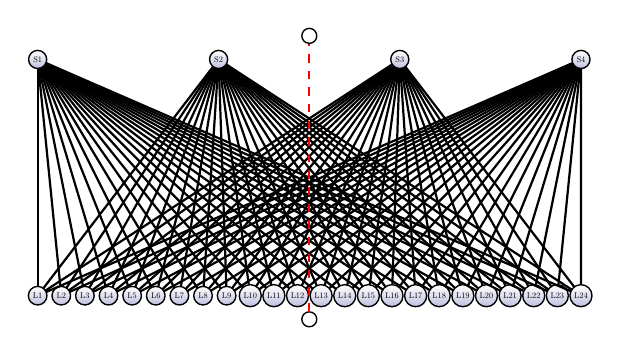
\begin{tikzpicture}[>=latex,line join=bevel,transform shape,scale=0.3]
	\GraphInit

	\Vertex[x=0,y=0,style=node]{L1}
	\Vertex[x=1,y=0,style=node]{L2}
	\Vertex[x=2,y=0,style=node]{L3}
	\Vertex[x=3,y=0,style=node]{L4}
	\Vertex[x=4,y=0,style=node]{L5}
	\Vertex[x=5,y=0,style=node]{L6}
	\Vertex[x=6,y=0,style=node]{L7}
	\Vertex[x=7,y=0,style=node]{L8}
	\Vertex[x=8,y=0,style=node]{L9}
	\Vertex[x=9,y=0,style=node]{L10}
	\Vertex[x=10,y=0,style=node]{L11}
	\Vertex[x=11,y=0,style=node]{L12}
	\Vertex[x=12,y=0,style=node]{L13}
	\Vertex[x=13,y=0,style=node]{L14}
	\Vertex[x=14,y=0,style=node]{L15}
	\Vertex[x=15,y=0,style=node]{L16}
	\Vertex[x=16,y=0,style=node]{L17}
	\Vertex[x=17,y=0,style=node]{L18}
	\Vertex[x=18,y=0,style=node]{L19}
	\Vertex[x=19,y=0,style=node]{L20}
	\Vertex[x=20,y=0,style=node]{L21}
	\Vertex[x=21,y=0,style=node]{L22}
	\Vertex[x=22,y=0,style=node]{L23}
	\Vertex[x=23,y=0,style=node]{L24}

	\Vertex[x=0,y=10,style=node]{S1}
	\Vertex[x=7.66,y=10,style=node]{S2}
	\Vertex[x=15.33,y=10,style=node]{S3}
	\Vertex[x=23,y=10,style=node]{S4}



	\Edge(L1)(S1)
	\Edge(L1)(S2)
	\Edge(L1)(S3)
	\Edge(L1)(S4)
	\Edge(L2)(S1)
	\Edge(L2)(S2)
	\Edge(L2)(S3)
	\Edge(L2)(S4)
	\Edge(L3)(S1)
	\Edge(L3)(S2)
	\Edge(L3)(S3)
	\Edge(L3)(S4)
	\Edge(L4)(S1)
	\Edge(L4)(S2)
	\Edge(L4)(S3)
	\Edge(L4)(S4)
	\Edge(L5)(S1)
	\Edge(L5)(S2)
	\Edge(L5)(S3)
	\Edge(L5)(S4)
	\Edge(L6)(S1)
	\Edge(L6)(S2)
	\Edge(L6)(S3)
	\Edge(L6)(S4)
	\Edge(L7)(S1)
	\Edge(L7)(S2)
	\Edge(L7)(S3)
	\Edge(L7)(S4)
	\Edge(L8)(S1)
	\Edge(L8)(S2)
	\Edge(L8)(S3)
	\Edge(L8)(S4)
	\Edge(L9)(S1)
	\Edge(L9)(S2)
	\Edge(L9)(S3)
	\Edge(L9)(S4)
	\Edge(L10)(S1)
	\Edge(L10)(S2)
	\Edge(L10)(S3)
	\Edge(L10)(S4)
	\Edge(L11)(S1)
	\Edge(L11)(S2)
	\Edge(L11)(S3)
	\Edge(L11)(S4)
	\Edge(L12)(S1)
	\Edge(L12)(S2)
	\Edge(L12)(S3)
	\Edge(L12)(S4)
	\Edge(L13)(S1)
	\Edge(L13)(S2)
	\Edge(L13)(S3)
	\Edge(L13)(S4)
	\Edge(L14)(S1)
	\Edge(L14)(S2)
	\Edge(L14)(S3)
	\Edge(L14)(S4)
	\Edge(L15)(S1)
	\Edge(L15)(S2)
	\Edge(L15)(S3)
	\Edge(L15)(S4)
	\Edge(L16)(S1)
	\Edge(L16)(S2)
	\Edge(L16)(S3)
	\Edge(L16)(S4)
	\Edge(L17)(S1)
	\Edge(L17)(S2)
	\Edge(L17)(S3)
	\Edge(L17)(S4)
	\Edge(L18)(S1)
	\Edge(L18)(S2)
	\Edge(L18)(S3)
	\Edge(L18)(S4)
	\Edge(L19)(S1)
	\Edge(L19)(S2)
	\Edge(L19)(S3)
	\Edge(L19)(S4)
	\Edge(L20)(S1)
	\Edge(L20)(S2)
	\Edge(L20)(S3)
	\Edge(L20)(S4)
	\Edge(L21)(S1)
	\Edge(L21)(S2)
	\Edge(L21)(S3)
	\Edge(L21)(S4)
	\Edge(L22)(S1)
	\Edge(L22)(S2)
	\Edge(L22)(S3)
	\Edge(L22)(S4)
	\Edge(L23)(S1)
	\Edge(L23)(S2)
	\Edge(L23)(S3)
	\Edge(L23)(S4)
	\Edge(L24)(S1)
	\Edge(L24)(S2)
	\Edge(L24)(S3)
	\Edge(L24)(S4)

	\Vertex[x=11.5,y=-1,style=invis,NoLabel=True]{MBBb}
	\Vertex[x=11.5,y=11,style=invis,NoLabel=True]{MBBt}

	\SetUpEdge[color=red,style=dashed]
	\Edge(MBBb)(MBBt)

      \end{tikzpicture}

    \end{center}
 
  }


  \frame{
    \frametitle{MBB vs Client BW - Clos}
    \begin{itemize}
      \item Bisection line cuts 2 of 4 links per leaf switch (48 total links cut)
      \pause\item 12 switches per half * 16 clients = 192 clients
      \pause\item 192:48 => 4:1
    \end{itemize}

  }

\section{Multi-path Ethernet and TCP/IP}
  \frame{

    \frametitle{Multi-path Ethernet and TCP/IP}
    \begin{itemize}
      \item<1-> Current efforts are underway to create multi-path options for more-common Ethernet and TCP/IP networks
      \item<2-> Some approaches:
      \begin{itemize}
	\item<2-> ECMP - Equal Cost Multi-Path Routing (layer 3)
	\begin{itemize}
	  \item<2-> Several layer 3 routing protocols support ECMP, including OSPF, IS-IS, and EIGRP
	\end{itemize}
	\item<3-> TRILL - Transparent Interconnection of Lots of Links - Multi-path layer-2 Ethernet\footnote<3->{The best reference I'm aware of is \emph{Introduction to Trill} by Radia Perlman and Donald Eastlake, available at \url{http://www.ipjforum.org/?p=582}}
      \end{itemize}
    \end{itemize}

  }

\section{Conclusions}
  \frame{
    \frametitle{What do I need to learn from this?}

    \begin{itemize}
      \item<2-> Not everything is Ethernet and TCP/IP
      \item<3-> A Tree-like topology may not be the best arrangement for a specific application, especially in data centers
      \item<4-> You absolutely \emph{must} understand the communication patterns of your application, in order to select the correct technology and topology
      \item<5-> What you're used to doing now, may change in the future
    \end{itemize}

  }


\section{Questions}

  \frame{
    \frametitle{Questions?}
    Any questions?
  }




\end{document}
